\chapter{Literature Review \label{chap:3_LiteratureReview}}

    % I could consult Candeloro2017Voronoi Literature Review

    In this chapter, we discuss the related studies, identifying their main contributions related to the development of global and local guidance systems for \ac{USV}. 
    The focus of this chapter is to highlight commonly used guidance methods, and explain in detail \ac{COLREGS}-compliant collision avoidance techniques presented in the literature.
    
    \section{Literature Review}

    %%%%%%%%%%%%%%%%%%%%%%%%%%%%%%%%%%%%%%%%%%%% Larson2006Autonomous
    \subsection{Larson 2006 Autonomous}
    Larson \etal~\cite{Larson2006Autonomous} explore the usage of A* in combination with \ac{VO}\footnote{In robotics and motion planning, a velocity obstacle, commonly abbreviated VO, is the set of all velocities of a robot that will result in a collision with another robot at some moment in time, assuming that the other robot maintains its current velocity.} \cite{Fiorini1998Motion} as path planner for global guidance. A* is used to avoid stationary obstacles, and \ac{VO} is used to avoid dynamic obstacles such as other vessels. The navigation is based on waypoints, and the global guidance system is responsible for the continuous modification of existing waypoints route to plan around obstacles detected with long-range sensors, such as \ac{AIS}, \ac{ARPA} contacts, and nautical charts. The \ac{AIS} system receives position, speed, and course data broadcasts from other marine vessels with compatible systems. The \ac{ARPA} system is capable of creating tracks using radar contacts and can calculate the tracked object's course, speed, and \ac{CPA}\footnote{Closest Point of Approach refers to the positions at which two dynamically moving objects reach their closest possible distance. \ac{CPA} is an important calculation for collision avoidance.}, thereby knowing whether there is a risk of collision with other ships or moving obstacles. Nautical charts can provide information about water depth, land heights, coastline, safe ways, navigational hazards, tides, currents, and human-made structures such as harbors, buildings, and bridges. Nautical charts are used as basic information for running A* and definition of waypoints. \ac{AIS} and \ac{ARPA} are used as basic information for running \ac{VO} and definition of waypoints.
    
    For local guidance, Larson \etal~\cite{Larson2006Autonomous} combines the information provided by a perception system for the generation of a local world-model. The perception system for near-field obstacles detection is composed of \ac{MWR}, Stereo Vision, Monocular Camera, and \ac{LADAR}. When an obstacle is detected, the new trajectory is defined based on the local world-model and a behavior-based approach. There are three behaviors: keep the last planned path, collision avoidance path, and free-space path. The decision is made through a voting system where the collision avoidance behavior vote is two times heavier than the others (\ie 2:1:1) and generates paths in an arc format, as shown in Figure \ref{fig:Larson2006Autonomous_Arcs}. Figure \ref{fig:Larson2006Automated_Summary} present a summary of Larson \etal~ work, the green path is the initial trajectory determined through A*, the blue path is the corrected trajectory for the avoidance of dynamic obstacles detected, and the red dots show the predicted trajectory of each obstacle using the \ac{VO} method.
    
    \begin{figure*}[t!]
    \centering
    
        \begin{subfigure}[t]{0.35\textwidth}
            \centering
            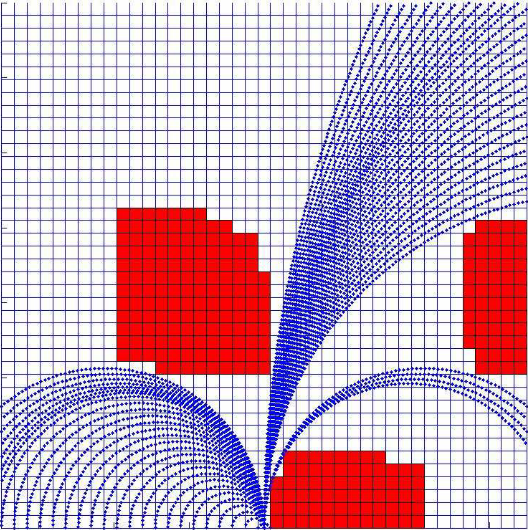
\includegraphics[width=0.75\textwidth]{figs/Chap3/Larson2006Autonomous_Arcs.png}
            \subcaption{Arc Path}
            \label{fig:Larson2006Autonomous_Arcs}
        \end{subfigure}%
        ~ 
        \begin{subfigure}[t]{0.6\textwidth}
            \centering
            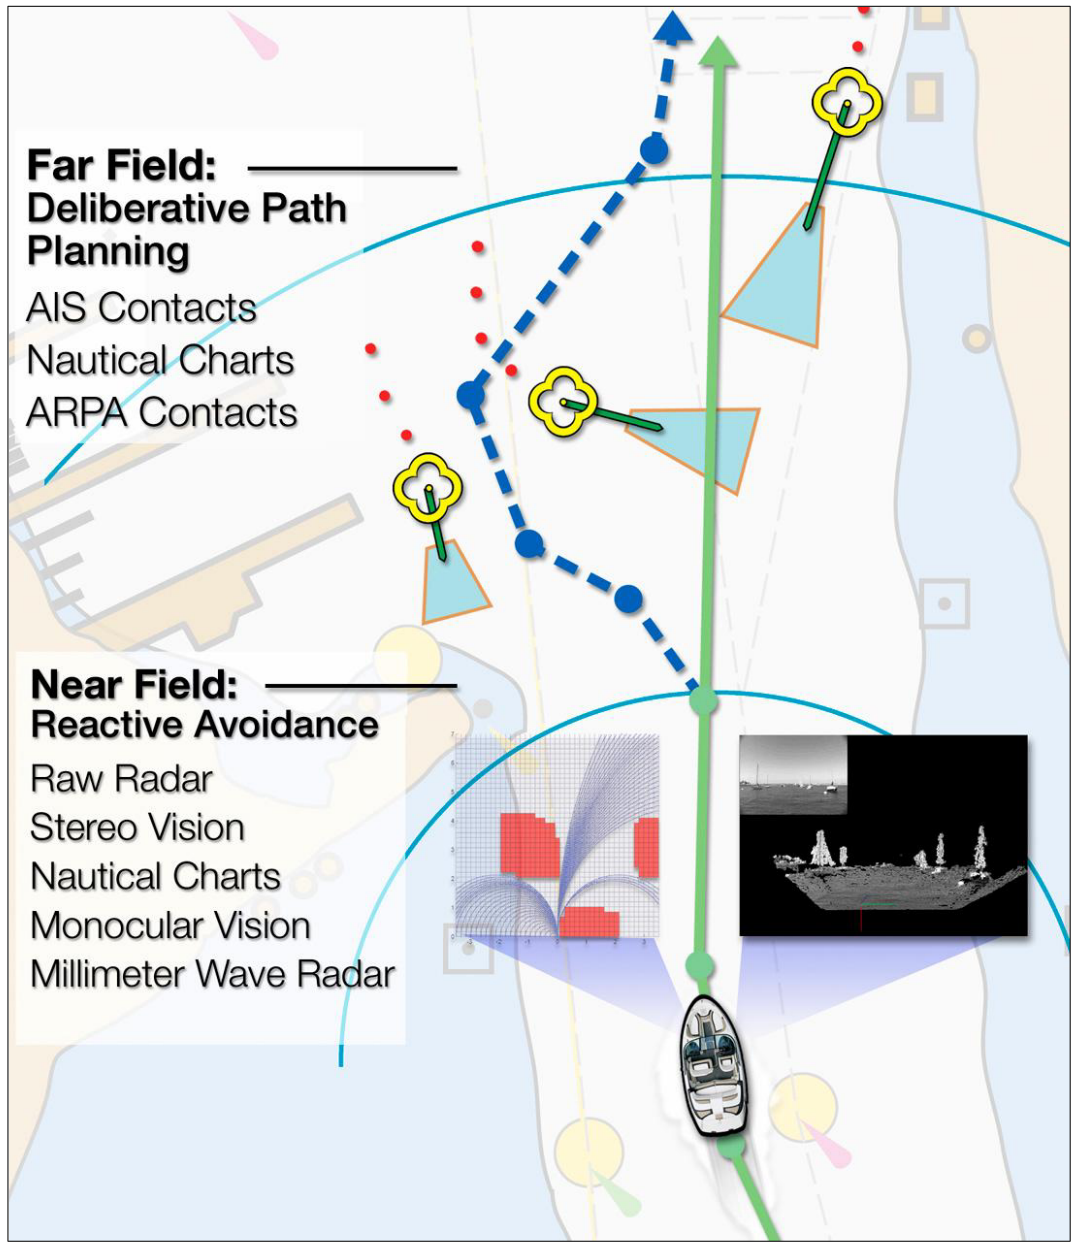
\includegraphics[width=\textwidth]{figs/Chap3/Larson2006Automated_Summary.png}
            \subcaption{Global Guidance Trajectories}
            \label{fig:Larson2006Automated_Summary}
        \end{subfigure}
        
    \caption{Guidance System Trajectories \cite{Larson2006Autonomous}}
    \end{figure*}
    %%%%%%%%%%%%%%%%%%%%%%%%%%%%%%%%%%%%%%%%%%%%
    
    %%%%%%%%%%%%%%%%%%%%%%%%%%%%%%%%%%%%%%%%%%%% Agrawal2015COLREGS
    \subsection{Agrawal 2015 COLREGS}
    Agrawal \etal~\cite{Agrawal2015COLREGS} present an \ac{USV} \ac{COLREGS}-compliant path planning strategy to follow another vessel in dynamic environments. Their solution is capable of predicting the target vessel motion, and then plan the route towards the target vessel while respecting the \ac{COLREGS}. 
    
    For collision avoidance, the system identifies \ac{COLREGS} conditions that apply to the current situation, in a specific time, considering nearby vessels and for each vessel is calculated the \ac{CPA}. If the \ac{CPA} is smaller than a threshold distance but not critical, the path is re-planned using A* with restriction in the search space for compliance to the \ac{COLREGS}.  When a critical distance is detected, the system re-plan using A* without restrictions in the search space. 
    
    For global guidance, the path is chosen based on the predicted motion for the target vessel using Monte-Carlo sampling of dynamically feasible and collision-free paths with fuzzy weights. The prediction is continuously optimized for a particular target by learning the necessary parameters for a 3-degree-of-freedom model of the vessel and its maneuvering behavior from its path history without any prior knowledge.
    
    For validation, they performed field tests on Panther Hollow Lake in Pittsburgh, PA, USA. They used 1.8m-long kayaks fitted with underwater-scooter motors on either side for propulsion, batteries, computers, compass, GPS, LIDAR scanners for obstacle detection, and RF receivers for manual control. The target-vessel was manually controlled at a speed of 1.7 m/s, and the presented test scenarios contain one civilian vessel that must be avoided. They successfully tested head-on and overtaking situations.
    %%%%%%%%%%%%%%%%%%%%%%%%%%%%%%%%%%%%%%%%%%%% 
    
    %%%%%%%%%%%%%%%%%%%%%%%%%%%%%%%%%%%%%%%%%%%%  Naeem2012COLREGS
    \subsection{Naeem 2012 COLREGS}
    For global guidance, Naeem \etal~\cite{Naeem2012COLREGS} use an A*-based algorithm, named \ac{DPSS}. 
    This method is based on a goal direction vector capable of reducing the search time by up to 50\%\cite{Yang2010Efficient}. The \ac{DPSS} algorithm produces waypoints around obstacles that form a smoother path with less sharp turns than A*. For local guidance, they use waypoint trajectory definition by \ac{LOS} \cite{Healey1993Multivariable}. Regarding \ac{COLREGS}-complaint collision avoidance, they present a manual biasing scheme consisting of always sailing towards the \ac{USV} starboard side to avoid collision situations with detected objects. They argue that avoiding obstacles always heading towards the starboard side makes the system compliant to the \ac{COLREGS}. However, this is not a good strategy since this action may lead to violation of other \ac{COLREGS} rules such as rule 10 that impose that navigation must respect \acf{TSS}.
    For dynamic obstacle detection, it is suggested the use of \ac{LIDAR} and cameras, and for the navigation system, they suggest the use of \ac{GPS}. The guidance system is evaluated through software simulation, where the control system uses a simple \ac{PID} for autopiloting.
        
    For collision avoidance, Naeem \etal~assume a \ac{COR} around each detected obstacle (shown in Figure \ref{fig:Naeem2012COLREGS_Trajectories_StaticObstacles}). For navigation Naeem \etal~assume a \ac{COA} around each waypoint. After the \ac{USV} enters the \ac{COA} the mission planner selects the next waypoint. Every time the distance between the \ac{USV} and an obstacle is less or equal than the \ac{COR}, the local guidance system becomes responsible for path plan generation. The system addresses collision avoidance for both dynamic and stationary obstacles. Figure \ref{fig:Naeem2012COLREGS_Trajectories_StaticObstacles} shows the generated trajectories using \ac{LOS} and \ac{DPSS} for avoid collision with static obstacles. Moreover, Figure \ref{fig:Naeem2012COLREGS_Trajectories_DynamicObstacles} shows a \ac{COLREGS}-compliant collision avoidance scenario, with dynamic obstacles.
    
    \begin{figure}[H]
    \centering
    
        \begin{subfigure}[b]{0.5\textwidth}
            \centering
            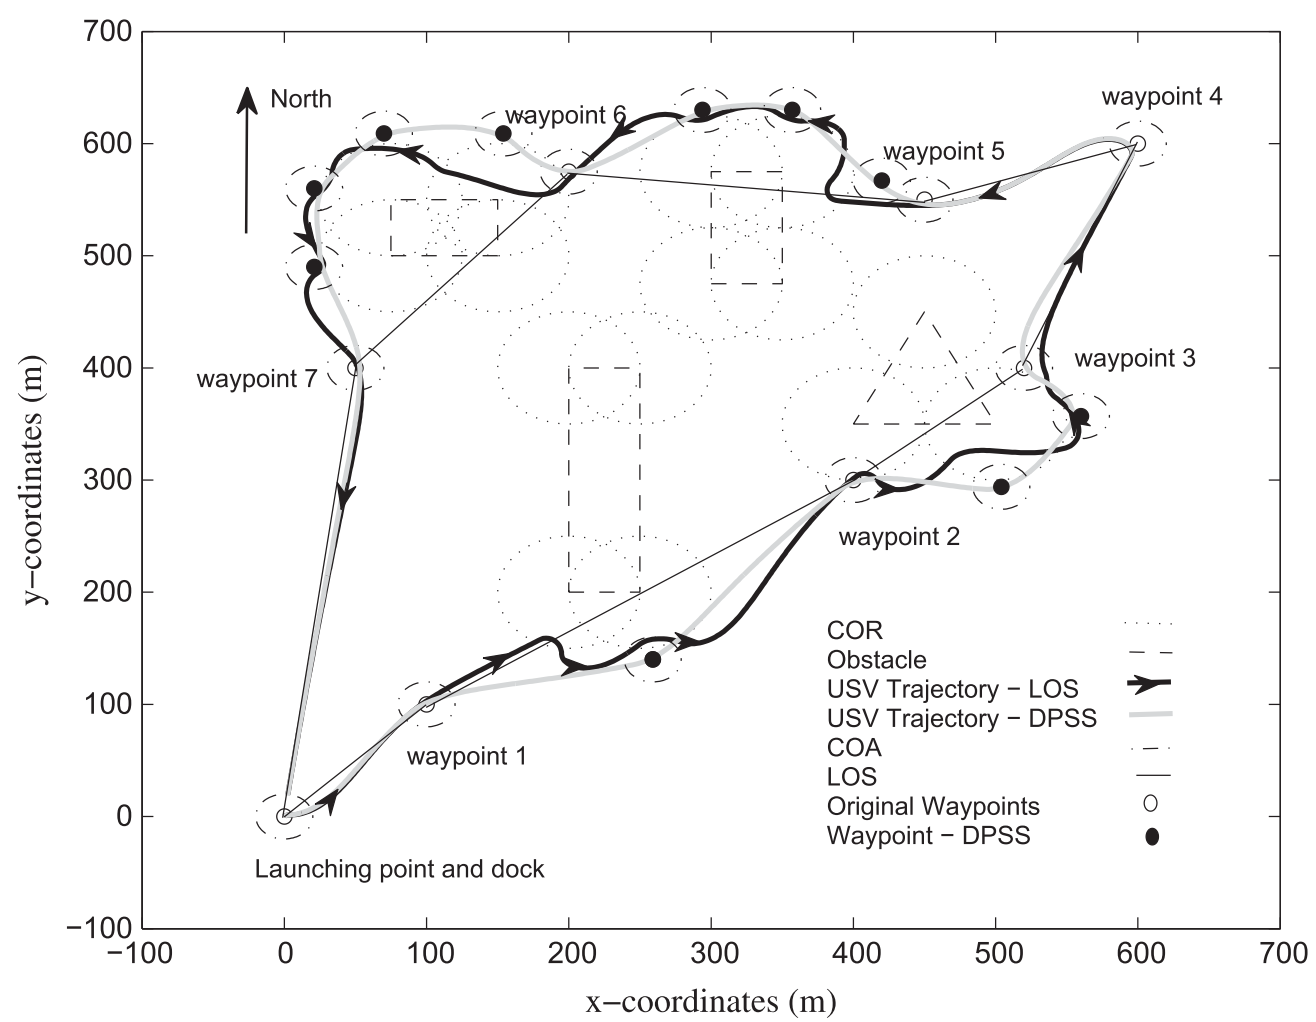
\includegraphics[width=\textwidth]{figs/Chap3/Naeem2012COLREGS_Trajectories_StaticObstacles.png}
            \caption{Static Obstacles}
            \label{fig:Naeem2012COLREGS_Trajectories_StaticObstacles}
        \end{subfigure}
        \begin{subfigure}[b]{0.4\textwidth}
            \centering
            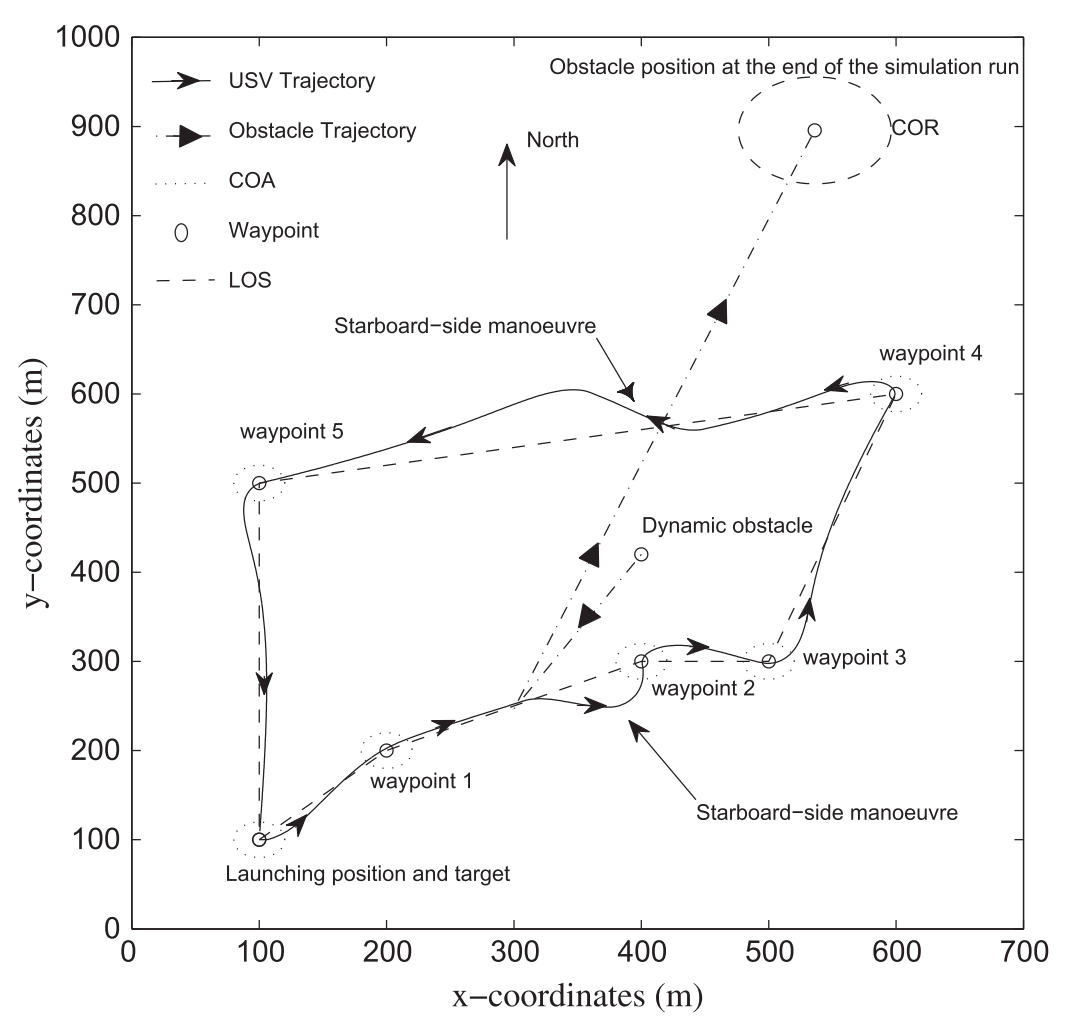
\includegraphics[width=\textwidth]{figs/Chap3/Naeem2012COLREGS_Trajectories_DynamicObstacles.png}
            \caption{Dynamic Obstacles}
            \label{fig:Naeem2012COLREGS_Trajectories_DynamicObstacles}
        \end{subfigure}
    
    \caption{Obstacles Avoidance Simulations \cite{Naeem2012COLREGS}}
    \label{fig:Naeem2012COLREGS_Trajectories}
    \end{figure}
    %VJ Explique a figura e o que é cada coisa na legenda e no texto.
    %%%%%%%%%%%%%%%%%%%%%%%%%%%%%%%%%%%%%%%%%%%% 
    
    %%%%%%%%%%%%%%%%%%%%%%%%%%%%%%%%%%%%%%%%%%%%  Campbell2013Automatic
    \subsection{Campbell 2013 Automatic}
    For obstacle avoidance, Campbell \etal~\cite{Campbell2013Automatic} present a system composed of a unit to predict the next position of detected obstacles. They use the \ac{CPA} method, assuming that detected obstacles will keep proceeding in their current velocities, this method finds the closest distance between encountering vessels at some time in the future. Moreover, a sampling interval is determined for updating the calculated distance. If the closest predicted distance is less than the acceptable range, the module advises a change in direction when an approaching threat is confirmed. The perception system is composed of a Microsoft HD video camera for object detection and identification and an Acuity laser range finder, so the basic information necessary for obstacle detection is extracted through the analysis of the data captured by the perception system. Moreover, the trajectory of the obstacles are predicted using Equations~\ref{eq:X} and \ref{eq:Y},
    \begin{equation}
    \label{eq:X}
    X = X_p + \int V cos(\psi)dt
    \end{equation}
    \begin{equation}
    \label{eq:Y}
    Y = Y_p + \int V sin(\psi)dt,
    \end{equation}
    where the pair \textit{X} and \textit{Y} is the predicted position, the pair $X_p$ and $X_y$ is the current position, and $\psi$ is current heading angle
    
    For global guidance, the system uses A*, and for local guidance, they use a modification of A*, named \ac{R-RA*}. The focus of this work is on describing the local guidance system. The \ac{R-RA*} method consists of having the path generated by A* as the base, and then perform iterative changes in the path to avoid collisions applying constraints to the search space. Path changes are performed in a local scope. The constraining is done on each iteration through the evaluation of the nodes in the search space and the addition of unwanted nodes to the A* closed list. That is, positions that violate the \ac{COLREGS} are marked as belonging to the closed list. This way, A* will not consider those nodes. The world is locally represented using a grid. A core assumption of the method is that \ac{USV}s can always determine other vessels' heading and velocity. The system uses this information for the calculation of the \ac{CPA}. The navigation system is composed by GPS and gyrocompass. Every time the distance between the \ac{USV} and the \ac{CPA} is shorter than the minimum acceptable distance, the local guidance system, with \ac{R-RA*} is activated. For system evaluation, they performed virtual simulations using the Virtual Sailor Simulator\footnote{Papini I. Virtual Sailor Software. SimSquared Ltd. Ship Simulator Shareware, 1999–2017. http://www.hangsim.com/virtual-sailor/}.
    %%%%%%%%%%%%%%%%%%%%%%%%%%%%%%%%%%%%%%%%%%%% 
    
    %%%%%%%%%%%%%%%%%%%%%%%%%%%%%%%%%%%%%%%%%%%%  Naus2013Idea
    \subsection{Nauss 2013 Idea}
    In Naus \etal~\cite{Naus2013Idea} the global guidance system uses A* for path planning. 
    Static data about the environment (\ie~topography, coastline, and safe way) is extracted from electronic navigational charts, and dynamic data (\ie~position of other ships) is extracted from \ac{DGPS}\footnote{Differential Global Positioning Systems (DGPS) are enhancements to the Global Positioning System (GPS) which provide improved location accuracy, in the range of operations of each system, from the 15-meter nominal GPS accuracy to about 10 cm in case of the best implementations.}, \ac{AIS}, and \ac{ARPA} sensors. This information is used to generate a map representation of the world and the sequential execution of the A* to determine the path to be followed by the \ac{USV}. This paper does not address the problem of collision avoidance for local guidance.
    %%%%%%%%%%%%%%%%%%%%%%%%%%%%%%%%%%%%%%%%%%%% 
    
    %%%%%%%%%%%%%%%%%%%%%%%%%%%%%%%%%%%%%%%%%%%%  Annamalai2013Comparison
    \subsection{Annamalai 2013 Comparison}
    Annamali \etal~\cite{Annamalai2013Comparison} focus on developing a control system but discuss the usage of a waypoint \ac{LOS} scheme \cite{Healey1993Multivariable} for global guidance. The \ac{USV} tries to go straight ahead from its current position until the next waypoint. For waypoint, following the control system was composed of a \ac{MPC} autopilot. In order to decide whether a waypoint has been reached or not, the guidance system considers a \ac{COA} around each waypoint. The suggested \ac{COA} radius is equal to the length of the vessel. The navigation system is equipped with \ac{GPS} for the determination of the current localization. For the determination of the current heading of the \ac{USV}, they combine the information provided by three electronic compasses (TCM2, HMR3000, and KVH-C100). For evaluation, the system was tested in simulated scenarios. This paper does not address the problem of local guidance.
    %%%%%%%%%%%%%%%%%%%%%%%%%%%%%%%%%%%%%%%%%%%% 
    
    %%%%%%%%%%%%%%%%%%%%%%%%%%%%%%%%%%%%%%%%%%%%  Lee2004Fuzzy
    \subsection{Lee 2004 Fuzy}
    Lee \etal~\cite{Lee2004Fuzzy} propose the use of \ac{VFF}\cite{Borenstein1989Real} for \ac{USV} \ac{COLREGS}-compliant collision avoidance. They present the \ac{MVFF} method, a modification of the traditional \ac{VFF} algorithm based on fuzzy logic. The focus is on the determination of the desired \ac{USV} heading angle $\Psi_d$ components. The geometric terms proposed consist of track-keep $\Psi_{tk}$, and collision avoidance angles $\Psi_{ca}$. 
    % VJ: usage vs use, no difference: less characters to type... #ficadica
    % VJ: mathematical components proposed? Acho melhor reescrever isso.
    The \ac{USV} route is defined by waypoints, where the path between consecutive waypoints is considered a straight line. However, movements that distance the \ac{USV} from the desired path may happen, for example, when a collision avoidance movement is required. Therefore, \ac{USV} motion strategy considers a combination of go towards the goal/next waypoint behavior and keep on tracking behavior. The heading angle mainly defines the motion of the \ac{USV}. Lee \etal~define the following formula for the desired heading angle:
    % VJ: eu resscrevi um pouco do parágrafo pois estava redundante. Explico: waypoints são pontos que devem ser seguidos. Desnecessário escrever isso.
    % VJ: Você está esquecendo de colocar virǵulas entre conectivos repetidamente. Cuidado redobrado ao iniciar frases.
    % VJ: Não é apenas desejável a combinação. Sem ela o robô pode não atingir o objetivo. Por isso eles combinaram os ângulos.
    % VJ Acho que os parágrafos acima e abaixo estão confusos e podem ser melhorados. Acima reescrever "The heading angle mainly defines the motion of the \ac{USV}". O texto do parágrafo abaixo pode ser combinado com a reescrita acima
    \begin{equation}
    \Psi_d = \Psi_{tk} + \Psi_{ca}
    \end{equation}
    % VJ: Dica sobre fórmula. Pense sempre assim: o símbolo tal representa, é, xpto, enquanto o símbolo bla é, representa, depicts xpto. Ou seja Psi-tk é o ângulo entre ..., whule psi_ca é bla.  
    The $\Psi_{tk}$ angle is related to a combination of the virtual forces that attract the \ac{USV}, respecting a proportion, to the desired track, and towards the goal. The $\Psi_{ca}$ angle is defined using fuzzy logic after the detection of obstacle direction, orientation, distance, relative velocity, and position relative to the \ac{USV}. Each detected value is translated into a weight for fuzzy logic decision. 
    
    Figure \ref{fig:Lee2004Fuzzy_tkAngle} illustrates a scenario where the \ac{USV} is relatively far from the desired track and must go to the Waypoint 2, $\vec{e}_a$  and $\vec{e}_p$ are the virtual forces related to the $\Psi_{ca}$ angle. Figure \ref{fig:Lee2004Fuzzy_caAngle} shows a similar scenario, but the \ac{USV} must avoid the obstacle present. The collision avoidance angle guides the avoidance.
    \begin{figure}[H]
    \centering
        \begin{subfigure}[b]{0.5\textwidth}
            \centering
            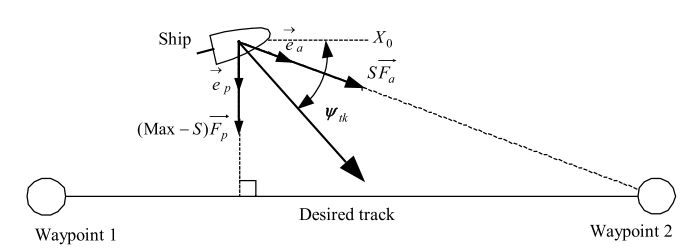
\includegraphics[width=\textwidth]{figs/Chap3/Lee2004Fuzzy_tkAngle.png}
            \caption{Track-Keep Angle}
            \label{fig:Lee2004Fuzzy_tkAngle}
        \end{subfigure}
        \begin{subfigure}[b]{0.4\textwidth}
            \centering
            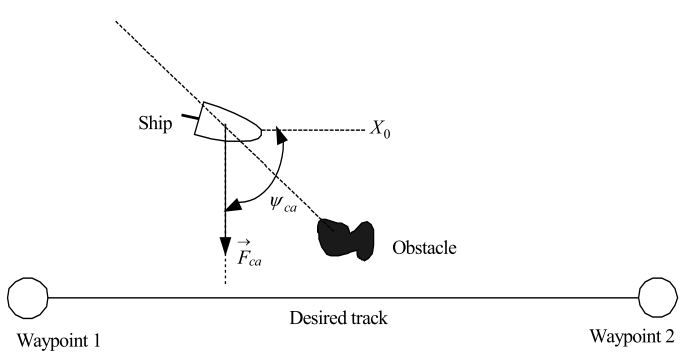
\includegraphics[width=\textwidth]{figs/Chap3/Lee2004Fuzzy_caAngle.png}
            \caption{Collision Avoidance Angle}
            \label{fig:Lee2004Fuzzy_caAngle}
        \end{subfigure}
    
    \caption{Vectors for angles determination \cite{Lee2004Fuzzy}}
    \label{fig:Lee2004Fuzzy_Angles}
    \end{figure}
    
    For simplicity, Lee \etal~\cite{Lee2004Fuzzy} assumed that the \ac{USV} is capable of only turn right. Simulation tests demonstrate that the presented method is applicable for implementation of \ac{COLREGS} rules 13, 14, 15, and 17 as presented in Figure \ref{fig:Lee2004Fuzzy_COLREGS_13_14_15_17}. 
    \begin{figure}[H]
    \centering
    
        \begin{subfigure}[b]{0.5\textwidth}
            \centering
            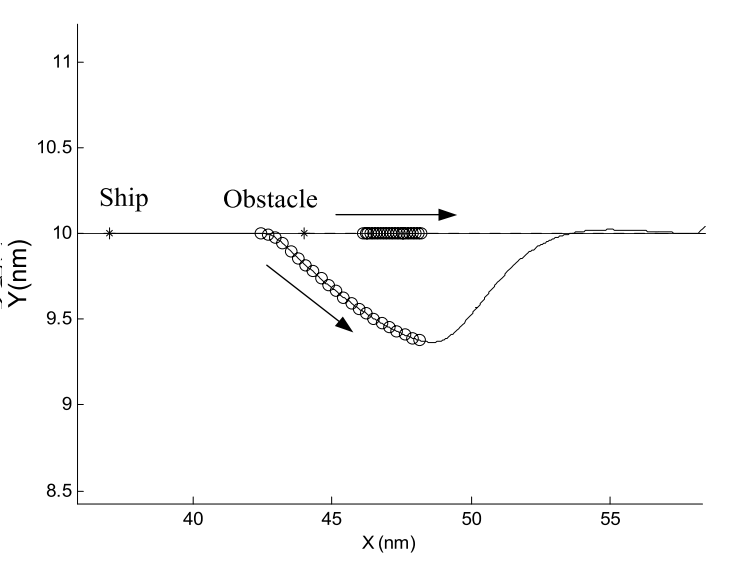
\includegraphics[width=\textwidth]{figs/Chap3/Lee2004Fuzzy_COLREGS13.png}
            \caption{\ac{COLREGS} rule 13}
            \label{fig:Lee2004Fuzzy_COLREGS13}
        \end{subfigure}
        \begin{subfigure}[b]{0.45\textwidth}
            \centering
            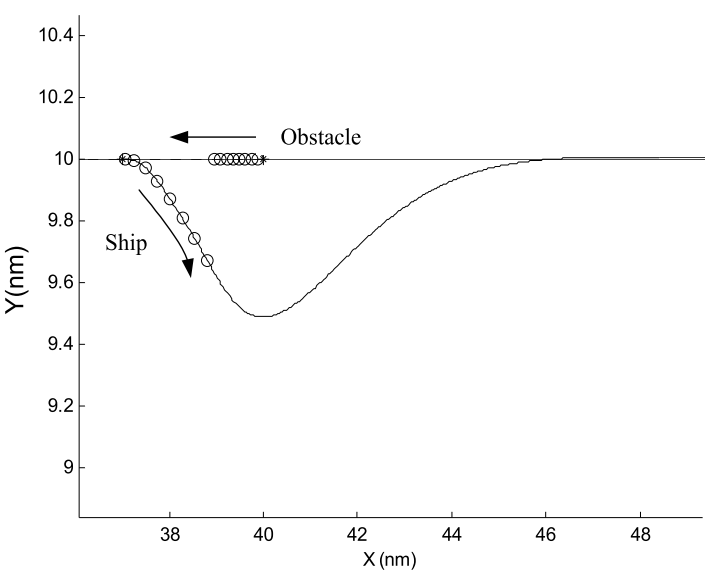
\includegraphics[width=\textwidth]{figs/Chap3/Lee2004Fuzzy_COLREGS14.png}
            \caption{\ac{COLREGS} rule 14}
            \label{fig:Lee2004Fuzzy_COLREGS14}
        \end{subfigure}
        
        \begin{subfigure}[b]{0.5\textwidth}
            \centering
            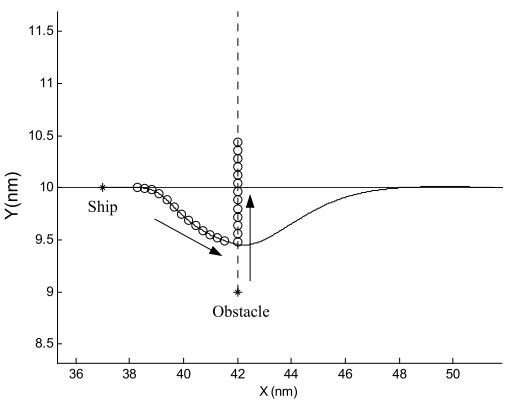
\includegraphics[width=\textwidth]{figs/Chap3/Lee2004Fuzzy_COLREGS15a.png}
            \caption{\ac{COLREGS} rule 15}
            \label{fig:Lee2004Fuzzy_COLREGS15}
        \end{subfigure}
        \begin{subfigure}[b]{0.45\textwidth}
            \centering
            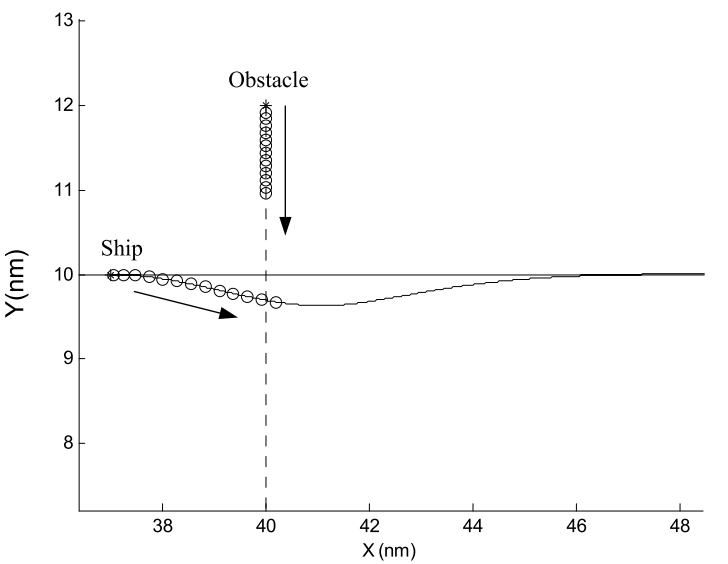
\includegraphics[width=\textwidth]{figs/Chap3/Lee2004Fuzzy_COLREGS18.png}
            \caption{\ac{COLREGS} rule 17}
            \label{fig:Lee2004Fuzzy_COLREGS18}
        \end{subfigure}
    
    \caption{Simulated tests \cite{Lee2004Fuzzy}}
    \label{fig:Lee2004Fuzzy_COLREGS_13_14_15_17}
    \end{figure}
    %%%%%%%%%%%%%%%%%%%%%%%%%%%%%%%%%%%%%%%%%%%%
    
    %%%%%%%%%%%%%%%%%%%%%%%%%%%%%%%%%%%%%%%%%%%% Kuwata2014Safe
    \subsection{Kuwata 2014 Safe}
    Kuwata \etal~\cite{Kuwata2014Safe} present a \ac{COLREGS}-compliant local guidance system based on \ac{VO} capable of addressing static and dynamic obstacles. Detection of dangerous situations is done through analyses of the \ac{CPA} and the geometric constraints presented in Figure~\ref{fig:Kuwata2014Safe_GeometricConstraints}, but the specific angles were not clearly defined. Environment information about static and dynamic obstacles are captured through a perception system composed of a radar, stereo cameras, and \ac{LIDAR}. On real-world tests, the \ac{USV} state is estimated by an onboard inertial navigation system. They discuss that \ac{VO} is an intuitive way to implement \ac{COLREGS} since \ac{VO} works on applying constraints to the \ac{USV} possible velocity space. Therefore, apply \ac{COLREGS} through \ac{VO} consists of applying some more constraints to the possible velocity space. They present the constraints used to implement \ac{COLREGS} rules 13 (overtaking), 14 (head-on), and 15 (crossing). For system evaluation, they executed real-world trials, and the \ac{USV} was exposed to around 30 scenarios with single and multiple vessel encounters. The \ac{USV} successfully acted on 24 maneuvers avoiding collision and did not respond safely to only one situation due to a vision sensor problem. They do not address global guidance system development.
    
    \begin{figure}[H]
        \centering
        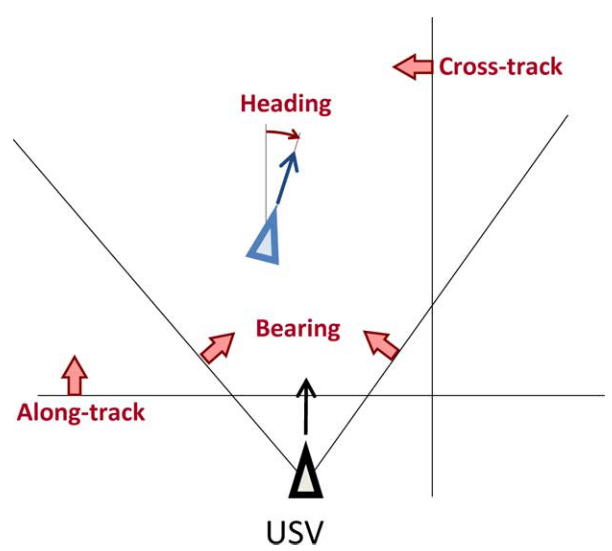
\includegraphics[scale=0.4]{figs/Chap3/Kuwata2014Safe_GeometricConstraints.png}
        \caption{Angle Analysis for Identification of Dangerous Situations \cite{Kuwata2014Safe}}
        \label{fig:Kuwata2014Safe_GeometricConstraints}
    \end{figure}
    
    %%%%%%%%%%%%%%%%%%%%%%%%%%%%%%%%%%%%%%%%%%%%
    
    %%%%%%%%%%%%%%%%%%%%%%%%%%%%%%%%%%%%%%%%%%%% Benjamin2004COLREGS
    For collision avoidance on local guidance, Benjamin \etal~\cite{Benjamin2004COLREGS} explore the use of a technique named Behavior-based Control and Multi-objective Action Selection. Different behaviors are defined corresponding to each possible situation, such as obstacle avoidance or keep the current mission. Each behavior defines objective functions that rates all possible actions concerning the corresponding \ac{COLREGS} rule. The decision space for vehicle action is defined based on variables such as course, speed, and intended-time. Tests are performed with four real kayaks. The navigation system is capable of determining its position from \ac{GPS}. Also, the \ac{USV} broadcasts their positions to each other. There is no specific detection system, after receiving position information, the \ac{USV} assumes that the \ac{GPS} information received corresponds to another \ac{USV} with which it must avoid collision.
    %%%%%%%%%%%%%%%%%%%%%%%%%%%%%%%%%%%%%%%%%%%%
    
    %%%%%%%%%%%%%%%%%%%%%%%%%%%%%%%%%%%%%%%%%%%%  Zhuang2011Motion
    \subsection{Zhuang 2011 Motion}
    In Zhuang \etal~\cite{Zhuang2011Motion}, they declare the usage of an evolutionary path planner~\cite{Russel2003AI_GA} for global guidance but do not specify which one and do not define clearly if the system is capable of dealing with static and dynamic obstacles. For local guidance, they used the \ac{VO} method \cite{Fiorini1998Motion}. Dangerous situations can happen in different forms, head-on encounter, crossing, overtaking. For the identification of different situations, the system is based on geometric constraints with limits defined by angles related to the \ac{USV} heading. As shown in figure \ref{fig:Zhuang2011Motion_Sectors}, the \ac{USV} heading is the 0° angle, 15° from the \ac{USV} angle defines the head-on encounter sector. A crossing is defined 135° from \ac{USV} heading. The system is evaluated through software simulation, and the results presented show that the local guidance system is compliant to \ac{COLREGS} rules 14 and 15.
    
    \begin{figure}[H]
        \centering
        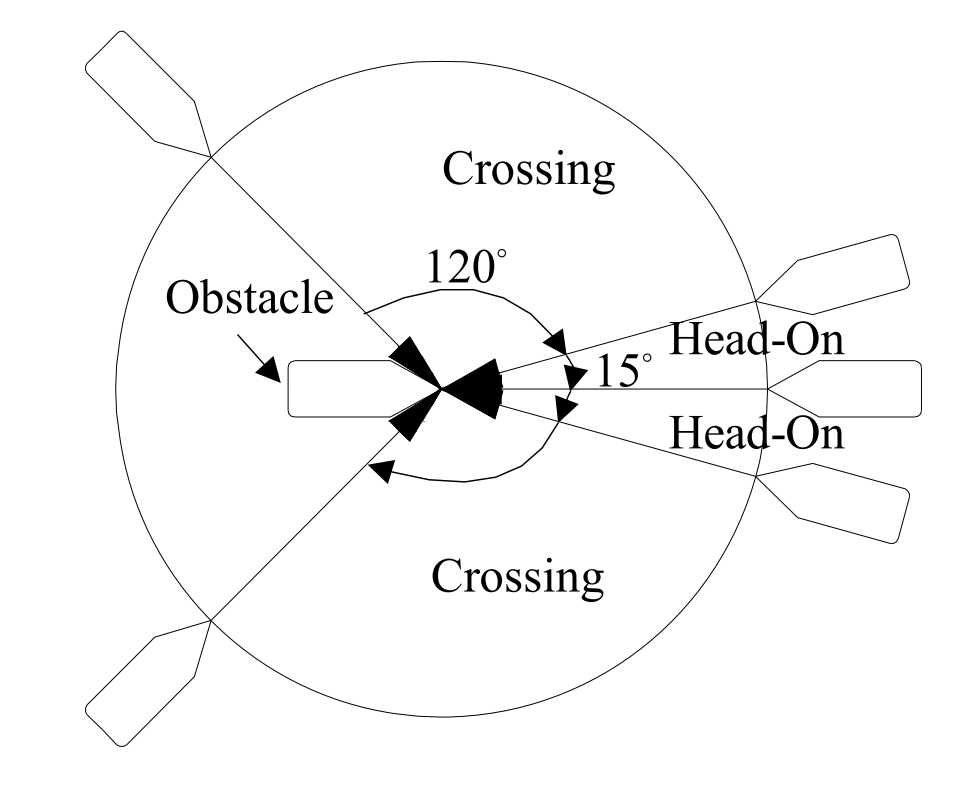
\includegraphics[scale=0.4]{figs/Chap3/Zhuang2011Motion_Sectors.png}
        \caption{Sectors for Identification of Dangerous Situation Type \cite{Zhuang2011Motion}}
        \label{fig:Zhuang2011Motion_Sectors}
    \end{figure}
    %%%%%%%%%%%%%%%%%%%%%%%%%%%%%%%%%%%%%%%%%%%%
    
    %%%%%%%%%%%%%%%%%%%%%%%%%%%%%%%%%%%%%%%%%%%% Svec2011
    \subsection{Svec 2011}
    For \ac{USV} trajectory definition, Svec \etal~\cite{Svec2011aAutomated, Svec2012Automated} present a automated guidance plan synthesis based on \ac{GP} method~\cite{Russel2003AI_GA}.
    % VJ explicar o que é isso bem rapidamente e atender o comentário acima do DJ :D
    % VJ Artigo relativamente importante, mas não me parece interessado em COLREGS.  Penso isso pelo termos usados: intruder... bloquear o avanço de intruder boats. Procede? Acho importante o artigo pois   existe um planejamento de alto nível.
    An initial version of a guidance plan is generated and then improved by detecting and fixing its shortcomings. The guidance plan is improved by data mining extraction of vehicle states of failure and then new iterations using \ac{GP}. Their solution is applied to the context of blocking the advancement of an intruder boat toward a valuable target. The guidance plan is represented as a composition of the navigation controller and a set of navigation plans.
    
    The navigation controller is composed of high-level navigation commands such as \textit{go-intruder-front}, \textit{turn-right}, \textit{turn-left}, and, \textit{go-straight}, conditional variables such as \textit{intruder-on-the-left/right/front/at-back}, \textit{intruder-has-target-on-the-left/right}, and \textit{usv-has-target-on-the-left/right}, standard \textit{boolean} values and operators such as \textit{if}, \textit{true}, \textit{false}, \textit{and}, \textit{or}, and \textit{not}, program blocks (seq2, seq3), and system commands (\textit{usv-sensor}, \textit{usv-velocity}, and \textit{usv-match-intruder-velocity})
    
    The navigation plan is composed of high-level navigation commands and program blocks.
    Leaves of the decision tree can be conditional variables or navigation commands.
    Inner nodes can be conditionals variables, navigation commands, or system commands.
    Figure \ref{fig:Svec2012Automated_GuidancePlanning} illustrates navigation controller and navigation plan.
    
    \begin{figure}[H]
        \centering
        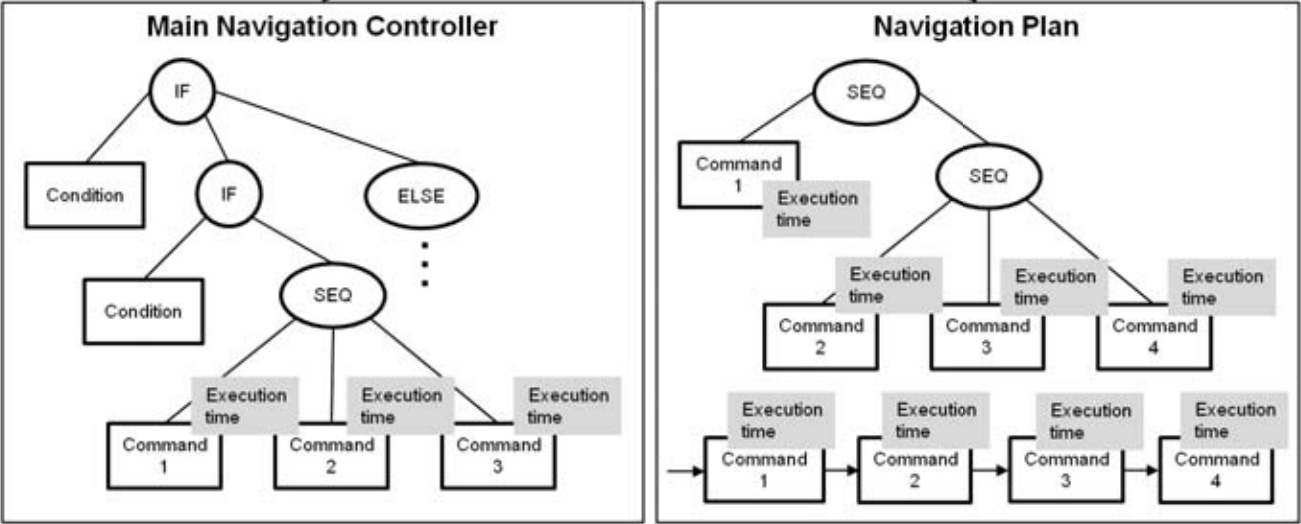
\includegraphics[scale=0.35]{figs/Chap3/Svec2012Automated_GuidancePlanning.png}
        \caption{Navigation controller and Navigation plan \cite{Svec2011aAutomated, Svec2012Automated}}
        \label{fig:Svec2012Automated_GuidancePlanning}
    \end{figure}
    %%%%%%%%%%%%%%%%%%%%%%%%%%%%%%%%%%%%%%%%%%%%
 
    %%%%%%%%%%%%%%%%%%%%%%%%%%%%%%%%%%%%%%%%%%%%  Soltan2009Trajectory
    \subsection{Soltan 2009 Trajectory}
    Soltan \etal~\cite{Soltan2009Trajectory} present the usage of \acp{ODE} for the approximation of the position of obstacles through the generation of elliptical fields around the obstacles. In this study, the \ac{USV} mission consists of following another target boat. The global guidance system tries to follow the target boat going towards it in a straight line. If any obstacle is detected, the local guidance system defines the trajectory around the obstacle considering the elliptical fields defined using \acp{ODE}. The evaluation of the system was done by simulation. They assumed that the \ac{USV} was capable of detecting any obstacle between the \ac{USV} and the target boat, in any range. Figure \ref{fig:Soltan2009Trajectory_SimulateTests_Ellipsses} shows two simulate scenarios where we can see elliptical fields for the approximation of 4 obstacles and the \ac{USV} trying to follow the target boat in 2 different scenarios.
    
    \begin{figure}[H]
        \centering
        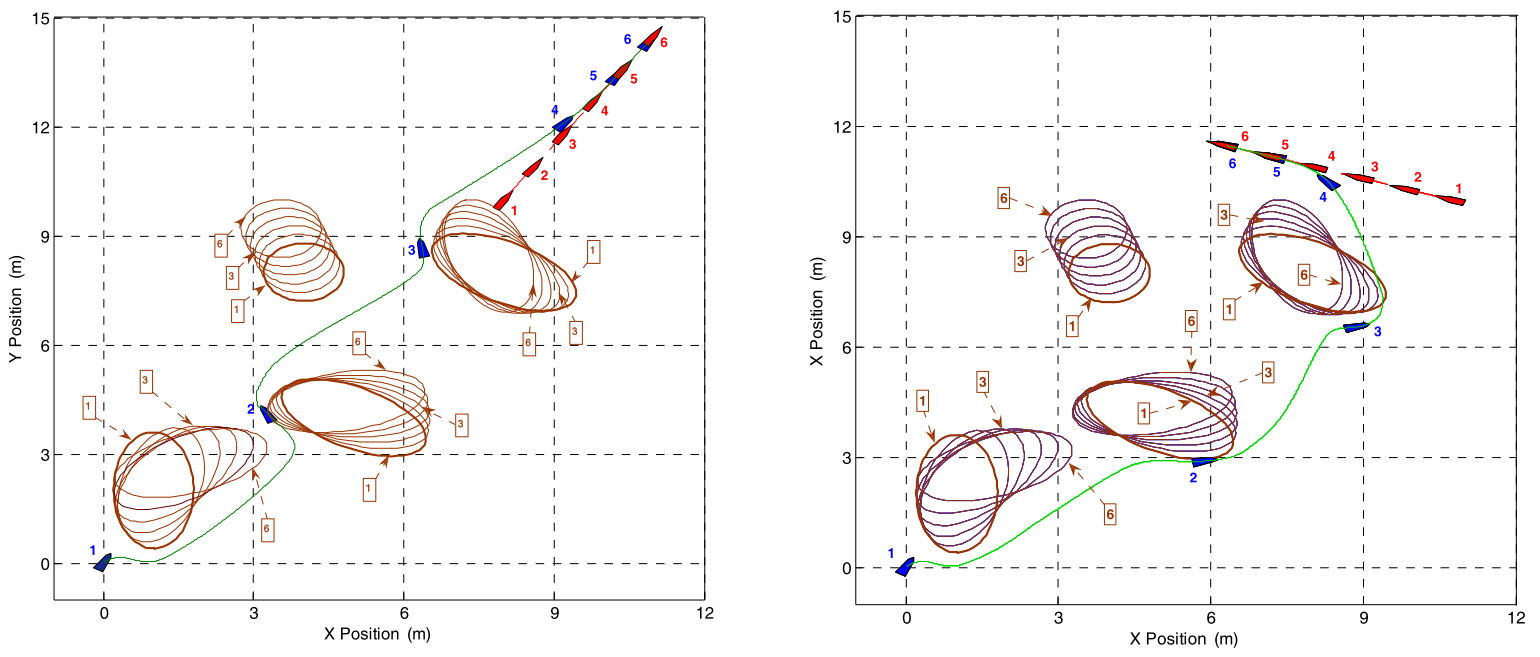
\includegraphics[scale=0.3]{figs/Chap3/Soltan2009Trajectory_SimulateTests_Ellipsses.png}
        \caption{Elliptical obstacles approximations \cite{Soltan2009Trajectory}}
        \label{fig:Soltan2009Trajectory_SimulateTests_Ellipsses}
    \end{figure}
    %%%%%%%%%%%%%%%%%%%%%%%%%%%%%%%%%%%%%%%%%%%% 
    
    %%%%%%%%%%%%%%%%%%%%%%%%% 
    %%%%%%%%%%%%%%%%%%%%%%%%% 2019 Reviews
    %%%%%%%%%%%%%%%%%%%%%%%%% 
    
    %%%%%%%%%%%%%%%%%%%%%%%%%%%%%%%%%%%%%%%%%%%% Abdelaal2017NMPC, Abdelaal2018Nonlinear 
    \subsection{Abdelaal 2017 NMPC}
    Abdelaal \etal~\cite{Abdelaal2017NMPC, Abdelaal2018Nonlinear} explore trajectory tracking controlling, based on \ac{MPC}. Trying to be COLREGS-compliant, their solution prioritizes maneuvering to the starboard side when in an encounter with obstacles, but this is not a suitable approach for real-world scenarios, as discussed before. They assume to be capable of detecting and identifying velocity, course, and length of other vessels, suggesting the use of \ac{LIDAR} and \ac{AIS} in tests on the field. The motion prediction of encountered vessels is made using a constant velocity model \cite{Rong2003Survey}. Obstacles are assumed to have a circular shape, and collision avoidance is translated into an inequality constraint, integrated into the controller design. The method is validated through software simulation using MATLAB.
    %%%%%%%%%%%%%%%%%%%%%%%%%%%%%%%%%%%%%%%%%%%%
    
    %%%%%%%%%%%%%%%%%%%%%%%%%%%%%%%%%%%%%%%%%%%% Benjamin2004COLREGS
    \subsection{Benjamin 2004 COLREGS}
    Benjamin \etal~\cite{Benjamin2004COLREGS} were pioneers in presenting a detailed discussion about the appliance of \ac{COLREGS} to USVs. Beyond, they present an overview of the "COLREGS project," showing simulation and field test modeling. Their strategy consisted of using a behavior-based control for the integration of \ac{COLREGS}-compliant collision avoidance and mission accomplishment.
    
    For \ac{COLREGS}-compliant global guidance, the output of each behavior is an objective function that rates all possible actions concerning the corresponding \ac{COLREGS}. So, they use interval programming to solve the multi-objective optimization problem. The \ac{COLREGS} behaviors rate possible vehicle actions in a decision space defined by the decision variables course, speed, and intended-time. Then, a not clearly defined shortest-path algorithm is run.
    
    For validation, they performed the test in simulation and field tests. In simulation, the controlled vehicle knows its own position perfectly, as well as the position and trajectory of all other moving vessels. They present the behavior related to the head-on situation. In the in-water experiments, the vehicle knows its position from GPS, and each vehicle broadcasts its GPS position to each other. Their experiment was performed using four 10-foot kayaks equipped with on-board computers running Linux and Mission Oriented Operating Suite\cite{MOOS}, GPS, compass, and a not clearly defined commercially available bathymetry map for the definition of free space.
    %%%%%%%%%%%%%%%%%%%%%%%%%%%%%%%%%%%%%%%%%%%%
    
    %%%%%%%%%%%%%%%%%%%%%%%%%%%%%%%%%%%%%%%%%%%% Huang2019Generalized 
    \subsection{Huang 2019 Generalized}
    Recently, some improvements have been made considering multi-ships dynamics. For example, Huang et al. \cite{Huang2019Generalized} present multi-vessel collision avoidance systems using an extension of the Velocity Obstacle algorithm, namely Generalized Velocity Obstacle, for local planning. Through software simulation, it is proved that the system is capable of avoiding multiple risks encounters with other vessels considering changes on course and speed and attending \ac{COLREGS} when possible. For \ac{COLREGS}-compliance, the system uses hard-port turn decision. Moreover, the authors argue that the system is suitable for both autonomous and officer support.
    
    \section{Literature Discussion}
    
    %% Grammarly 100/100
    In this section, we briefly discuss important aspects related to the development of \ac{USV} guidance and collision avoidance systems presented in the literature. Based on the read studies, we can have a glance about the relevance of A*, \ac{LOS}, and \ac{VO} for \ac{USV} guidance and the focus on addressing avoidance of overtaking, head-on, and crossing collision situations.
    
    
    \subsection{Guidance}
    
    %% Grammarly 100/100
    In general, guidance based on path planning requires addressing both stationary and dynamic obstacles. Regarding real-world-tested work, guidance requires an accurate world model and robust methods to avoid detected obstacles. World representation is done using cost maps and information is collected through nautical charts~\cite{Larson2006Autonomous}, electronic charts~\cite{Naus2013Idea}, \ac{ARPA} contacts~\cite{Larson2006Autonomous}, and \ac{AIS}~\cite{Abdelaal2017NMPC}. The usage of these two last allow path planning for global guidance to consider not only stationary obstacles but moving obstacles also. Regarding the location and orientation of the \ac{USV} itself, the literature presented the usage of GPS~\cite{Benjamin2004COLREGS} and compasses~\cite{Annamalai2013Comparison}. Based on our literature review we identified the following methods for global and local planning
    
    \begin{enumerate}
    
        %% Grammarly 100/100
        \item Regarding global planning we identified the usage of the following methods: \ac{VO}~\cite{Larson2006Autonomous, Kuwata2014Safe, Zhuang2011Motion, Huang2019Generalized}, A*~\cite{Naeem2012COLREGS, Campbell2012Review_COLREGs, Naus2013Idea} e genetic programming~\cite{Svec2012Automated, Svec2011aAutomated}. The works that presented A* and VO for global planning achieved proper behavior, being capable of planning and avoiding collision in the scenarios presented by the authors. At the same time, the usage of optimization methods (\ie~genetic programming) implied limitations due to the high cost for real-time applications. 
        
        %% Grammarly 100/100
        \item Regarding local planning we identified the usage of the following methods: A*\cite{Larson2006Autonomous, Campbell2013Automatic, Agrawal2015COLREGS}, \ac{VO}~\cite{Larson2006Autonomous, Huang2019Generalized}, \ac{LOS}~\cite{Naeem2012COLREGS}, and Virtual Force Field~\cite{Lee2004Fuzzy}. Also, the review presented by Liu \etal~\cite{Liu2016Unmanned} indicates the usage of potential fields~\cite{Healey2007Collaborative, Soltan2009Trajectory}. Regarding \ac{COLREGS} compliance, the heuristics solutions were based on search space restriction while the solutions presented by  Naeem~\etal~\cite{Naeem2012COLREGS}, Lee~\etal~\cite{Lee2004Fuzzy}, consisted in perform a hard turn to the starboard side in every detected encounter between vessels. We consider this is not a good approach since this action may lead to violation of other \ac{COLREGS} rules such as rule 10 that impose that navigation must respect \acf{TSS}.
        
    \end{enumerate}
    
    Collision avoidance is performed mostly with an architecture composed of two subsystems, one deliberative and other reactive. Deliberative systems are based on well-known maps and are implemented through optimization and heuristics methods. Reactive systems run online, are based on real-time collected data from \ac{LIDAR}~\cite{Agrawal2015COLREGS}, \ac{SONAR}~\cite{Candeloro2017Voronoi}, and cameras\cite{Kuwata2014Safe} and requires more intelligent systems since they must be compliant to protocols such as the \ac{COLREGS}. 
    
    Based on the literature, the identification of \ac{COLREGS} situation can be made through the calculation of the bearing angle~\cite{Kuwata2014Safe}\footnote{We use it in our system and explain it in chapter~\ref{chap:4_COLREGS_Compliant_Guidance_System}}. Some authors present the usage of \ac{CPA}~\cite{Campbell2013Automatic} for anticipated detection of \ac{COLREGS} situation while other authors present pure reactive approach.
    
    Relevant work that applied and tested their techniques on real-world situations worked on using a well-known method, such as A* and \ac{VO}, and applied some constraints on the search space of action to make them \ac{COLREGS}-complaint \cite{Kuwata2014Safe, Campbell2013Automatic}. 
    The \ac{COLREGS}-complaint systems presented in the literature were evaluated through software simulation~\cite{Soltan2009Trajectory, Abdelaal2017NMPC, Benjamin2004COLREGS, Lee2004Fuzzy} as much as tested on field~\cite{Agrawal2015COLREGS, Benjamin2004COLREGS, Kuwata2014Safe}.
    
    One of the challenges involving \ac{COLREGS} is related to the fact that the rules were defined expecting a large amount of human intuition and experience to fulfill gaps and non-objective rules descriptions. For example, the vague definition of angles, and distances that must be respected generate non-standard parameters definition. Studies explicitly declare that these parameters were empirically defined after several tests \cite{Larson2007Advances}, but these definitions not necessarily solve the problem for \ac{USV} of different sizes and capabilities, generating a generalization problem.
    
    %AMA favor usar https://www.grammarly.com/. usa esse user moraesfg@gmail.com e essa senha 'moraes65'. depois de usar, apaga o arquivo gerado.
    
    
    
    
    
    % \section{Literature Discussion}
    
    % In this section, we briefly discuss important aspects related to the development of \ac{USV} guidance and collision avoidance systems presented in the literature. Table \ref{tab:RelatedWork_Summary} presents a summary of the methods used for implementation of guidance system path planners and the addressed \ac{COLREGS} rules. Based on read studies, we can have a glance about the relevance of A*, \ac{LOS} and \ac{VO} for \ac{USV} guidance and the focus on addressing avoidance of overtaking, head-on and crossing collision situations.
    
    % \begin{table}[H]
    % \caption{Literature guidance methods and applied COLREGS rules summary}
    % \label{tab:RelatedWork_Summary}
    % \begin{tabular}{l|c|c|c|c}
    % \hline
    % \multicolumn{1}{c}{Studies}            & Global & Local & Hybrid & \multicolumn{1}{c}{COLREGS-compliance (Rules)}   \\ \hline
    % \hline
    % \cite{Larson2006Autonomous}                     & A*              & Arcs           &                 &                                                          \\
    % \cite{Naeem2012COLREGS}                         & DPSS            & LOS            &                 & 6, 8,  14, and 15, and 16                                \\
    % \cite{Campbell2013Automatic}                    & A*              & R-RA*          &                 & 6, 8, 13, 14, 15, and 16                                 \\
    % \cite{Naus2013Idea}                             & A*              &                &                 &                                                          \\
    % \cite{Annamalai2013Comparison}                  & LOS             &                &                 &                                                          \\
    % \cite{Lee2004Fuzzy}                             &                 & VFF + Fuzzy    &                 & 6, 8, 13, 14, 15, 16, and 17                             \\
    % \cite{Kuwata2014Safe}                           &                 & VO             &                 & 6, 8, 13, 14, 15, and 16                                 \\
    % \cite{Benjamin2006Method}                       &                 & Behavior       &                 & 14                                                       \\
    % \cite{Zhuang2011Motion}                         & Evolutionary    & VO             &                 & 14, 15, and 16                                           \\
    % \cite{Svec2011aAutomated, Svec2012Automated}    &                 &                & GP              &                                                          \\
    % \cite{Soltan2009Trajectory}                     &                 &                & ODE             &                                                          \\ \hline
    % \end{tabular}
    % \end{table}
    
    % In addition to the presented studies, the survey presented by Liu \etal~\cite{Liu2016Unmanned} highlights the following studies and methods for guidance and collision avoidance: 
    % A* \cite{Svec2011Trajectory, Svec2012USV}; 
    % \ac{LOS} \cite{Breivik2008Straight, Caccia2008Basic, Caccia2005Sampling, Desa2007Small, Fredriksen2006Global, Naeem2012Integrated, Peng2013Adaptive, Sharma2013Genetic, Xu2007Multi};
    % Potential Fields \cite{Healey2007Collaborative, Soltan2009Trajectory}; and
    % Near-field reactive control \cite{Larson2007Advances}.
    
    % % Discussion about guidance
    % % VJ Darlan, as 2 subsections abaixo estão curtas e misturadas em termos de conteúdo. Vc explica path planning for guidance... quando o título é guidance. Depois vc explica que collision avoidance requer blah blah. Talvez remover as subsections desta sessão te ajude a deixar o texto mais fluído.
    % \subsection{Guidance}
    % In general, Guidance based on path planning requires to address both stationary and dynamic obstacles. Focusing on real-world tested work, guidance requires accurate world model and robust methods to avoid obstacles detected. World representation is done using occupancy grid and information is collected through nautical charts, electronic charts, \ac{ARPA} contacts, and \ac{AIS} contacts. The usage of these two last allow path planning for global guidance to consider not only stationary obstacles but moving obstacles also.
    
    % % Discussion about collision avoidance
    % \subsection{Collision Avoidance}
    % Collision avoidance is performed mostly with an architecture composed of two subsystems, one deliberative and other reactive. Deliberative systems are based on well-known maps and are implemented through optimization and heuristics methods. Reactive systems run online, are based on real-time collected data from \ac{LIDAR}, \ac{SONAR}, and cameras and requires more intelligent systems since they must be compliant to protocols such as the \ac{COLREGS}.
    
    % % Discussion about \ac{COLREGS}
    % % Vc implementa as COLREGS? Ou um método de planejamento para seguir COLREGS?
    % % DJ: Done
    % \subsection{COLREGS}
    % \ac{COLREGS}-compliant methods implementation involves definition of USV geometric constraints as shown in Figure \ref{fig:Zhuang2011Motion_Sectors} and \acf{CPA} for identification of which possible dangerous situation must be avoided. 
    % Relevant work that applied and tested their techniques on real-world situations worked on using a well-known method, such as A* and \ac{VO}, and applied some constraints on the search space of action to make them \ac{COLREGS}-complaint \cite{Kuwata2014Safe, Campbell2013Automatic}. 
    % In general, the \ac{COLREGS}-complaint systems presented in the literature were evaluated through software simulation without being tested on field guiding real boats.
    
    % One of the challenges involving \ac{COLREGS} is related to the fact that the rules were defined expecting a large amount of human intuition and experience to fulfill gaps and non-objective rules descriptions. 
    % % parece que vc vai citar outros quando vc diz one of the challenges, mas o parágrafo termina
    % For example, the vague definition of angles, and distances that must be respected generate non-standard parameters definition. Studies explicitly declare that these parameters were defined after several tests \cite{Larson2007Advances} but these definitions not necessarily solve the problem for \ac{USV} of different size and capabilities, generating a problem of generalization.
    
    % %AMA favor usar https://www.grammarly.com/. usa esse user moraesfg@gmail.com e essa senha 'moraes65'. depois de usar, apaga o arquivo gerado.
    
    % Relacionada a guidance, apresentamos abaixo as técnicas apresentadas na literatura para global planning e local planning. 

    % \begin{enumerate}
    %     \item Global planning: A partir da revisão da litaratura apresentada, observamos a utilização dos métodos \ac{VO}~\cite{Larson2006Autonomous, Kuwata2014Safe, Zhuang2011Motion, Huang2019Generalized}, A*~\cite{Naeem2012COLREGS, Campbell2012Review_COLREGs, Naus2013Idea} e genetic programming~\cite{Svec2012Automated, Svec2011aAutomated}. The works that presented A* and VO for gloabl planning, achieved suitable behavior, being capable to plan and avoid collision in the scenarios presented by the authors. While, the usage of optimization methods (\ie genetic programming) implied limitations due to the high cost for real-time application. 
        
    %     \item Local planning: A partir da revisão da literatura apresentada, observamos a utilização dos métodos A*\cite{Larson2006Autonomous, Campbell2013Automatic, Agrawal2015COLREGS}, \ac{VO}~\cite{Larson2006Autonomous, Huang2019Generalized}, \ac{LOS}~\cite{Naeem2012COLREGS}, and Virtual Force Field~\cite{Lee2004Fuzzy}. In addition, the review presented by Liu \etal~\cite{Liu2016Unmanned} indicate the usage of potential fields~\cite{Healey2007Collaborative, Soltan2009Trajectory}. Regarding COLREGS compliance, the heuristics solutions were based on search space restriction while the solutions presented by  Naeem~\etal~\cite{Naeem2012COLREGS}, Lee~\etal~\cite{Lee2004Fuzzy}, consisted in perform a hard turn to the starboard side in every detected encounter between vessels.
    % \end{enumerate}